\documentclass[12pt,a4paper]{article}

\usepackage[utf8]{inputenc}
\usepackage[T1]{fontenc}
	% if you don't use \usepackage[T1]{fontenc},
    % - Words containing accented characters (ö,...) cannot be automatically hyphenated,
    % - You cannot properly copy-and-paste such words from the output (DVI/PS/PDF),
    % - Characters like the pipe sign, less than and greater sign give unexpected results in text.
\usepackage{lmodern}  % Vector Fonts even when using T1 !
\usepackage[ngerman]{babel}
\usepackage[dvipsnames,cmyk]{xcolor} % xcolor and more colornames, cymk for printing
\usepackage{cmap} % pro­vides char­ac­ter map ta­bles, which makes PDFs search­able and copy-able (I don't see a difference yet!!!)
\usepackage{graphicx}   % for /includegraphics command
\usepackage{cancel}		% for making a stroke through a calculation
%\usepackage{tensor}    % enables indices in all for corners of a variable
%\usepackage{pdflscape}	% rotate site by 90° with \begin{landscape}
\usepackage{url}		% for \url{} command to not get problems with :\\ and other symbols
\usepackage{hyperref}	% for labellinks and more
\usepackage[labelfont=bf]{caption} % allows captions in non-figure environments with \captionof and \captionsetup
\usepackage{siunitx}    % SI units paper conform with \SI{3}{\nano\seconds}

\usepackage[backend=bibtex]{biblatex}% ist default style=numeric,
\usepackage{bibgerm}
\addbibresource{literatur.bib}


\usepackage{listings}   % source code listings
\definecolor{mygreen}{rgb}{0,0.6,0}
\definecolor{mygray}{rgb}{0.5,0.5,0.5}
\definecolor{mymauve}{rgb}{0.58,0,0.82}

\lstset{ %
  backgroundcolor=\color{white},   % choose the background color; you must add \usepackage{color} or \usepackage{xcolor}
  basicstyle=\footnotesize,        % the size of the fonts that are used for the code
  breakatwhitespace=false,         % sets if automatic breaks should only happen at whitespace
  breaklines=true,                 % sets automatic line breaking
  captionpos=b,                    % sets the caption-position to bottom
  commentstyle=\color{mygreen},    % comment style
%  deletekeywords={...},            % if you want to delete keywords from the given language
  escapeinside={\%*}{*)},          % if you want to add LaTeX within your code
  extendedchars=true,              % lets you use non-ASCII characters; for 8-bits encodings only, does not work with UTF-8
  %frame=single,                    % adds a frame around the code
  keepspaces=true,                 % keeps spaces in text, useful for keeping indentation of code (possibly needs columns=flexible)
  keywordstyle=\color{blue},       % keyword style
  morekeywords={*,...},            % if you want to add more keywords to the set
  numbers=left,                    % where to put the line-numbers; possible values are (none, left, right)
  numbersep=5pt,                   % how far the line-numbers are from the code
  numberstyle=\tiny\color{mygray}, % the style that is used for the line-numbers
  rulecolor=\color{black},         % if not set, the frame-color may be changed on line-breaks within not-black text (e.g. comments (green here))
  showspaces=false,                % show spaces everywhere adding particular underscores; it overrides 'showstringspaces'
  showstringspaces=false,          % underline spaces within strings only
  showtabs=false,                  % show tabs within strings adding particular underscores
  stepnumber=1,                    % the step between two line-numbers. If it's 1, each line will be numbered
  stringstyle=\color{mymauve},     % string literal style
  tabsize=2,                       % sets default tabsize to 2 spaces
  title=\lstname                   % show the filename of files included with \lstinputlisting; also try caption instead of title
}

% allow direct input of greek letters and similar. Also add some own unicode chars additionally to uniinput
\usepackage{uniinput}
\DeclareUnicodeCharacter{2208}{\ensuremath{\in}}
\DeclareUnicodeCharacter{2115}{\ensuremath{\mathbb N}}
\DeclareUnicodeCharacter{2124}{\ensuremath{\mathbb Z}}
\DeclareUnicodeCharacter{2192}{\ensuremath{\rightarrow}}

%%%%%%%%%%%%%%%%%%%%%%%%%%%%%%%%%%%%%%%%%%%%%%%%%%%%%%%%%%%%%%%%%%%%%%%%%%%%%%%%
% own commands and formattings 
%%%%%%%%%%%%%%%%%%%%%%%%%%%%%%%%%%%%%%%%%%%%%%%%%%%%%%%%%%%%%%%%%%%%%%%%%%%%%%%%

\setlength\parindent{0pt} % stop indenting every paragraph by 1cm. It looks awful!

% some mathematical functions
\newcommand{\arsinh}{\text{arsinh}\,}
\newcommand{\arcosh}{\text{arcosh}\,}
\newcommand{\arcoth}{\text{arcoth}\,}
\newcommand{\artanh}{\text{artanh}\,}
\newcommand{\atan}{\text{atan}\,} %short for ArcTan
\newcommand{\asin}{\text{asin}\,}
\newcommand{\acos}{\text{acos}\,}

\newcommand{\de}{\text{d}}                      % integration d
\newcommand{\const}{\text{\small const.}}
\renewcommand{\nabla}{\overrightarrow{\bigtriangledown}}
\newcommand{\laplace}{\bigtriangleup}
\newcommand{\dalembert}{\square}
\newcommand{\affects}[1]{\overset{\downarrow}{#1}} % arrow pointing down to variables affected bei DOP
\newcommand{\fpart}[2]{\frac{\partial #1}{\partial #2}} 
\newcommand{\ftdif}[2]{\frac{\de #1}{\de #2}}      % short for e.g. df/dx
\newcommand{\slfrac}[2]{\left.#1\middle/#2\right.} % slanted fraction like 3/4 (slash sign)

\usepackage[backend=bibtex]{biblatex}% ist default style=numeric,
\usepackage{bibgerm}
\addbibresource{literatur.bib}


%%%%%%%%%%%%%%%%%%%%%%%%%%%%%%%%%%%%%%%%%%%%%%%%%%%%%%%%%%%%%%%%%%%%%%%%%%%%%%%%
% main part
%%%%%%%%%%%%%%%%%%%%%%%%%%%%%%%%%%%%%%%%%%%%%%%%%%%%%%%%%%%%%%%%%%%%%%%%%%%%%%%%

\begin{document}

\begin{titlepage}
\begin{center}
\rule{\textwidth}{3px}
\Huge{
Komplexpraktikum:\\
Paralleles Rechnen}\\[-12pt]
\rule{\textwidth}{3px}\\[3cm]

\vfill

\large
\begin{tabular}{rl}
	Protokoll von: & Maximilian Knespel\\
	Betreuer: & Dr. Bernd Trenkler
\end{tabular}\\[3cm]
{\large \today}
\end{center}
\end{titlepage}

\newpage

\tableofcontents
\newpage

%%%%%%%%%%%%%%%%%%%%%%%%%%%%%%%%%%%%%%%%%%%%%%%%%%%%%%%%%%%%%%%%%%%%%%%%%%%%

\section{Test-Setup}

%%%%%%%%%%%%%%%%%%%%%%%%%%%%%%%%%%%%%%%%%%%%%%%%%%%%%%%%%%%%%%%%%%%%%%%%%%%%

\subsection{Hardwarespezifikationen}

\begin{center}
	\centering
	\captionsetup{type=figure}
	\begin{minipage}{\linewidth}
		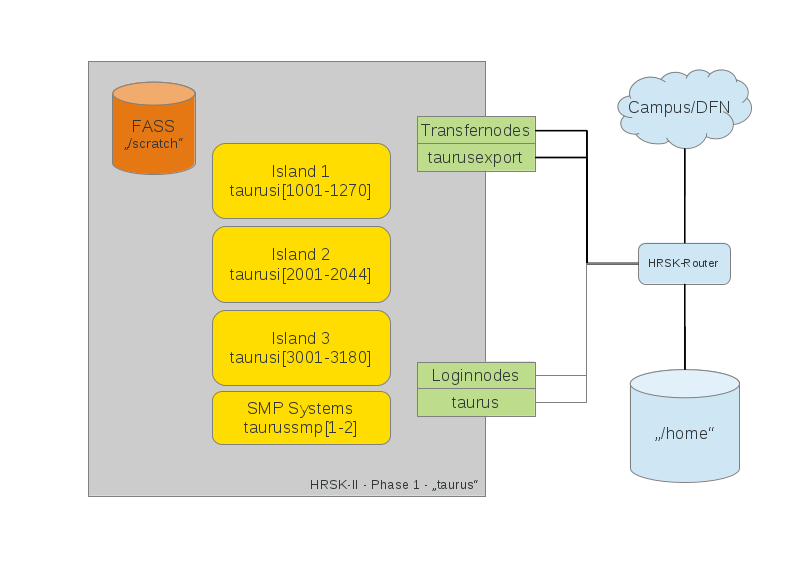
\includegraphics[width=\linewidth]{../systemlayout}
	\end{minipage}
	\captionof{figure}{Systemübersicht des Taurus-Clusters. }
	\label{fig:tauruslayout}
\end{center}

Insel 1\cite{tudhardwaretaurus}:
\begin{itemize}
	\item 270 Nodes: taurusi1[001-270]
	\item 2x Intel(R) Xeon(R) CPU E5-2690 (8 cores) @ 2.90GHz, MultiThreading Disabled
	\item 2 GB RAM per core (32 GB total): taurusi[1001-1220,1226-1229,1253-1254,1262-1263] (228 nodes)
	\item 4 GB RAM per core (64 GB total): taurusi[1221-1225,1230-1252] (28 nodes)
	\item 8 GB RAM per core (128 GB total): taurusi[1255-1261,1264-1270]  (14 nodes)
\end{itemize}

\begin{center}
\captionsetup{type=table}
\begin{tabular}{|l|c|}
	\hline
		\multicolumn{2}{|c|}{\textbf{Intel Xeon CPU E5-2690}} \\
	\hline
	\hline
	Architektur & Ivy Bridge (22nm) \\
	\hline
	Prozessortakt & 2900MHz \\
	\hline
	Thermal Design Power & 135 Watt \\
	\hline
	Kerne/Threads & 8/16 (Multithreading deaktiviert auf Taurus) \\
	\hline
	L1-Cache & 8 x 32 KB Instruction Cache \\
	         & 8 x 32 KB Data Cache \\
	\hline
	L2-Cache & 8 x 256 KB \\
	\hline
	L3-Cache & 20 MB \\
	\hline
	Turbotakt & 3800 MHz (1 core)\\
              & 3600 MHz (2 or 3 cores)\\
              & 3400 MHz (4 or 5 cores)\\
              & 3300 MHz (6 or more cores) \\
	\hline
\end{tabular}
	\captionof{table}{Ausgesuchte Leistungsmerkmale des Taurus Insel 1 Prozessors\cite{cpuworldxeon}}
\end{center}


%%%%%%%%%%%%%%%%%%%%%%%%%%%%%%%%%%%%%%%%%%%%%%%%%%%%%%%%%%%%%%%%%%%%%%%%%%%%%%%%

\subsection{Zeitmessung}

%%%%%%%%%%%%%%%%%%%%%%%%%%%%%%%%%%%%%%%%%%%%%%%%%%%%%%%%%%%%%%%%%%%%%%%%%%%%%%%%

Eine sehr portable Möglichkeit zur Zeitmessung ist mit der MPI-Standard-Funktion MPI\_Wtime() gegeben. Diese gibt die Sekunden seit einem nicht näher bestimmten Zeitpunkt als double zurück. Die Genauigkeit dieser Funktion kann man mit MPI\_Wtick() abfragen.
Die Auflösung von MPI\_Wtick scheint mit der C-internen Zeitauflösung CLOCKS\_PER\_SECOND und der dazugehörigen Zeitabfrage clock() übereinzustimmen. Hardware Zeitgeber sind folgende: 
\begin{itemize}
	\item PIT(PIC): ein Legacy Timer mit 1.193182 MHz, praktisch aber auf z.B. Linux nur 100Hz
%(http://telematics.tm.kit.edu/publications/Files/61/walter_ibm_linux_challenge.pdf)
	\item APIC: wird von Linux genutzt um 1µs-Zeitauflösung zu erreichen
	\item RTC: 2Hz bis 32768Hz
	\item HPET
	\item TSC: Zählt die Anzahl der CPU-Takte. Hat also die Frequenz der aktuellen CPU-Frequenz. Problematisch bei CPU-Stromsparmodi, die die CPU bei wenig Last runtertakten.
\end{itemize}
% Wie spreche ich alle mit Assembler an? Dann wären die Unterschiede auch klar, bzw. wo finde cih die auf den Boards ???

Für die Messung eines einzelnen Durchlaufs ist die Auflösung von MPI\_Wtime zu gering. Deswegen war es von der Aufgabenstellung angedacht über 100 Ping-Pong-Kommunikationen zu messen und dann die Zeit durch 200 zu teilen. Dies wurde gemacht.\\

Zusätzlich dazu wurde jedoch die Zeitmessung auch mittels RDTSC gemessen. Eine CPU-Funktion mit Opcode 0F31, die in 64-bit EDX:EAX die aktuelle Anzahl an Takten zurückgibt. Für eine korrekte Zeitmessung muss man noch verhindern, dass RDTSC Out-of-Order ausgeführt wird. Dies geschieht mit cpuid. \ref{http://www.strchr.com/performance_measurements_with_rdtsc} Eine andere nicht getestete Methode ist RDTSCP, was eine serieller RDTSC ist, da es auch die CPU ID abholt. Intel schlägt in seinen Dokumenten Volume 2 Chapter 4.2 RDTSC\ref{!!!} auch vor LFENCE vor RDTSC zu benutzen.\\

\begin{center}\begin{minipage}{0.75\linewidth}\begin{lstlisting}[language=C++]
uint64_t GetCPUCycle() {
    uint32_t lo,hi;
    asm volatile (
        ".intel_syntax noprefix \n"
        "xor eax,eax            \n"
        "cpuid                  \n"
        "rdtsc                  \n"
        ".att_syntax            \n"
        : "=d" (hi), "=a" (lo)  /* out */
        : /* no input */
        : "cc" /* cluttered registers */
    );
    return (uint64_t(hi) << 32) + uint64_t(lo);
}
\end{lstlisting}\end{minipage}
\end{center}

Der Vorteil an dieser Methode ist, dass man 100 einzelne Zeiten hat und daraus auch eine Standardabweichung berechnen kann, was auch getan wurde. Problematisch wäre auch die Anzahl der Takte zwischen zwei verschiedenen Cores zu vergleichen, da sie nicht synchronisiert sein müssen. Aber da wir nur Differenzen vergleichen ist das kein Problem.\\
Problematisch wäre jedoch, wenn der Scheduler den Thread während der Runtime auf einen anderen Core wechselt.  Seit OpenMPI Version 1.7.4 ist die Option "--bind-to core" jedoch default.\ref{https://github.com/open-mpi/ompi-release/blob/v1.7/NEWS}

Da man nur die Takte hat, braucht man noch die CPU-Taktrate. Diese wurde mittels eines einer gleichzeitigen Zeitmessung mittels MPI\_Wtime() und RDTSC über 10 Sekunden ermittelt. Die ermittelten Werte sind in Tabelle~\ref{tbl:freqs} aufgeführt.\\

\begin{center}
\captionsetup{type=table}
\begin{tabular}{|l|c|}
	\hline
	Nodename & Taktfrequenz \\
	\hline
	\hline
	'Same Node'  & $(2.899944 \pm 0.0000003)$ GHz \\
	'Other Node' & $(2.899927 \pm 0.0000003)$ GHz \\
	Home         & $(3.299817 \pm 0.0000003)$ GHz \\
	\hline
\end{tabular}
\captionof{table}{Die Unsicherheiten kommen rein aus der Dauer der Zeitmessung und könnten damit gegen 0 gehen für beliebig lange Zeiten. Es fehlen Unsicherheiten aus der Zeitmessung und die Varianz statistischer Fehler, die für beliebig lange Messung konstant und größer 0 bleiben wird. (!!! REDO with correct names)}
\label{tbl:freqs}
\end{center}

\newpage

%%%%%%%%%%%%%%%%%%%%%%%%%%%%%%%%%%%%%%%%%%%%%%%%%%%%%%%%%%%%%%%%%%%%%%%%%%%%

\section{Punkt-zu-Punkt-Kommunikation mit MPI}

%%%%%%%%%%%%%%%%%%%%%%%%%%%%%%%%%%%%%%%%%%%%%%%%%%%%%%%%%%%%%%%%%%%%%%%%%%%%

Ziel ist es die benötigte Zeit für eine Punkt-zu-Punkt Kommunikation zwischen zwei Prozessen zu vermessen.

\begin{center}\begin{minipage}{0.75\linewidth}\begin{lstlisting}[language=C++, caption={Ping-Kommunikation implementiert in C++. MPI_Send blockt bis die Daten das Ziel erreicht haben!}, label=lst:ping]
	if ( rank == 1 )
	    MPI_Recv( const_cast<uint8_t *>(msg), length, MPI_BYTE, 
	              rank-1, i, MPI_COMM_WORLD, MPI_STATUS_IGNORE );
	if (rank == 0) {
        /* sleep 1ms until receiving mechanism is set up => Benchmark *
         * takes 0.001*N_REPETITIONS*(N_LIN_UP_TO+N_LOG_VALUES) longer*/
        t0  = MPI_Wtime(); while( MPI_Wtime()-t0 < 0.001 ) {}
        t0  = MPI_Wtime();
        nc0 = GetCPUCycle();
        MPI_Send( const_cast<uint8_t *>(msg), length, MPI_BYTE,
                  rank+1, i, MPI_COMM_WORLD);
        nc1 = GetCPUCycle();
        t1  = MPI_Wtime();
	}
\end{lstlisting}\end{minipage}\end{center}

In Listing~\ref{lst:ping} wird die Zeit für eine Kommunikation gemessen, die bei kurzen Nachrichten unmessbar kurz ist. Es wurde auch nochmal kumulativ über 100 Ping-Pong-Kommunikationen gemessen:\\

\begin{center}\begin{minipage}{0.75\linewidth}\begin{lstlisting}[language=C++, caption={Kumulative Zeitmessunf für 100 Ping-Pong-Kommunikationen}, label=lst:ping-pong]
t0 = MPI_Wtime();
for (uint64_t i = 0; i < repetitions; i++) {
    if ( rank == 1 ) {
        MPI_Recv( const_cast<uint8_t *>(msg), length, MPI_BYTE,
                  rank-1, 0, MPI_COMM_WORLD, MPI_STATUS_IGNORE);
        MPI_Send( const_cast<uint8_t *>(msg), length, MPI_BYTE,
                  rank-1, 0, MPI_COMM_WORLD);
    } else if ( rank == 0 ) {
        MPI_Send( const_cast<uint8_t *>(msg), length, MPI_BYTE,
                  rank+1, 0, MPI_COMM_WORLD);
        MPI_Recv( const_cast<uint8_t *>(msg), length, MPI_BYTE,
                  rank+1, 0, MPI_COMM_WORLD, MPI_STATUS_IGNORE);
    }
    MPI_Barrier( MPI_COMM_WORLD ); //was used because of this Bug under Windows and Cygwin: http://www.open-mpi.org/community/lists/users/2014/10/25606.php
}
t1  = MPI_Wtime();

\end{lstlisting}\end{minipage}\end{center}

%Parameter und ausgewählte Level:
%\begin{itemize}
%	\item Nachrichtenlänge: 1...4150 Bytes, danach 1000 logarithmisch verteilte Werte bis zu 10Mb. (Redo (wo memcpy) with 300mb or even more by specifying more than 300mb max per processor with slurm ???)
%	\item Kommunikation: OpenMPI, memcpy
%	\item Zeitmessung: kumulativ, einzeln und nachträglich gemittelt
%	\item Zu sendende Daten: neue Zufallsdaten nach jedem Senden, nur einmal Zufallsdaten bei Programmstart erstellt
%	\item Messsystem: 2 Cores auf einem Node Taurus Insel 1, 2 Threads auf unterschiedlichen Nodes auf Taurus Insel 1, 2 Cores auf meinem Heim-PC (genauer Spezifikationen von RAM, CPU, ... der Rechner!!!)
%\end{itemize}
%
%Die Hintergedanken:
%
%
%Einflussfaktoren:
%\begin{itemize}
%	\item multithreads und paging -> nochmal exklusiv laufen lassen ???
%	\item cpu stromsparmodi
%	\item Programmversionen Taurus : OpenMPI 1.6.5 64-bit, gcc 4.9.1 64-bit
%	                        Heim-PC: OpenMPI 1.8.3 64-bit, gcc 4.8.3 64-bit
%	                 Vergessen OpenMPI 1.8.3 auf Taurus zu nehmen (1.6.5. ist default, warum), nochmal durchführen wegen bind-to core auch vergessen ???
%    \item Welcher Node genau. Vergessen zu dokumentieren. Nochmal durchführen ???
%\end{itemize}

%%%%%%%%%%%%%%%%%%%%%%%%%%%%%%%%%%%%%%%%%%%%%%%%%%%%%%%%%%%%%%%%%%%%%%%%%%%%%%%%

\subsection{Zwei Cores auf einem Node (local)}

%%%%%%%%%%%%%%%%%%%%%%%%%%%%%%%%%%%%%%%%%%%%%%%%%%%%%%%%%%%%%%%%%%%%%%%%%%%%%%%%

Bei Auftragung der Transfergeschwindigkeit über die logarithmische Nachrichtenlänge in Abb.\ref{fig:SameNode} zeichnet sich ein sättigender Anstieg ab, der dann bei ca. 6.3MB abzufallen scheint. (Wiederholung der Messung bis 100mb!!!) Diese Grenze liegt auf Größenordnung und unter der des L3-Caches von 20MB. Da der L3-Cache von den 8 Cores geteilt wird, kann es sein, dass der Rest des Caches mit anderen Dingen befüllt ist, z.b. durch das Betriebssystem oder OpenMPI, oder dass einfach der Prediction-Algorithm nicht den vollen Cache ausnutzen kann, wobei zweiteres bei dieser einfachen Anwendung unwahrscheinlich ist. (Wiederholen mit SLURM --exclusive !!!) Der erreichte Maximalwert der Transferrate ist \textbf{bei ca. 10GB/s, dies ist die Kommunikationsbandbreite}. Zumindest für OpenMPI Kommunikationen, siehe auch Kap.\ref{sct:memcpy}. \textbf{Es sollten keine Nachrichten größer 6.3MB verschickt werden.} Das ist ca. ein Drittel des L3-Caches.\\

\begin{center}
	\centering
	\captionsetup{type=figure}
	\begin{minipage}{0.6\linewidth}
		\includegraphics[width=\linewidth]{../01/SameNode.pdf}
	\end{minipage}
	\captionof{figure}{Transferraten in Abhängigkeit der Nachrichtenlänge. Bei der Erstellung der Benchmarkwerte wurde einmal mit den kurzen Nachrichten begonnen und einmal mit langen Nachrichten begonnen.}
	\label{fig:SameNode}
\end{center}

Im Vergleich 'shortest message first' vs. 'longest message first' ist eigtl. anzunehmen, dass es keine Unterschiede gibt. Leider wird aber nicht nach jeder Nachricht der komplette Zustand des PCs zurückgesetzt, sodass unbekannte Faktoren mitwirken können. Die Anfangsvermutung lag eigentlich im Caching: Wenn man mit großen Nachrichten anfängt, dann liegt schon ein Großteil der Nachrichten im Cache, vor allem, wenn man weiter zu Nachrichten kleiner der Cache-Größe geht. Fängt man jedoch mit den kleinen Nachrichten an, so ist möglicherweise nur ein Teil der Nachricht schon im Cache, während der Rest nachgeladen werden muss. So zumindest die Vermutung. Qualitativ wurde diese Annahme widerlegt: Die Transferraten für 'longest first' liegen fast immer \textbf{unter} denen von 'shortest first', es ist also langsamer. Das ist seltsam und steht auch im Widerspruch zu den Resultaten für Memcpy in Kap.\ref{sct:memcpy}. Andererseits würde es nur in den Grenzfällen, wo die Nachrichtenlänge gewechselt wurde, eine Rolle spielen.\\
Der Versuch sollte für memcpy und MPI\_Send wiederholt werden (!!!)\\

Der Bandbreiteneinbruch bei ca. 4000Byte ist bei allen bis auf MPI\_Wtime an der gleichen Stelle und scheint damit eine systematische Ursache zu haben. Z.b. eine bestimmte Cache-Größe oder eine Schwelle an der OpenMPI das Kommunikationsprotokoll ändert. Für eine genauere Lokalisierung auf +-1 Byte müsste die Messung an dieser Stelle mit mehr Messpunkten wiederholt werden (!!!).
Die andere Unstetigkeit bei 460KB für 'longest first' scheint zufällig zu sein, aber auch hier müsste die Messung für mehr Klarheit wiederholt werden (!!!).\\
Die Unstetigkeit bei 800kb tritt bei der Messung über 100 Vorgänge mit MPI\_Wtime \textbf{und} bei 'shortest first' auf und scheint damit nicht zufällig zu sein. Dass die Werte dann aber auf der Kurve für 'longest first' liegen, die schon eher hoch ging, spricht wieder für einen zeitlich zufälligen Fehler, z.b. dass die Taktrate sich verändert hat. Das würde aber nicht ganz erklären, warum MPI\_Wtime auch davon betroffen ist, außer wenn auch der Speicherbustakt davon betroffen ist.\\
Auch bei ca. 10kb springt 'MPI\_Wtime' ein wenig nach unten auf einer Art paralleln Kurvenverlauf\\

\begin{center}
	\centering
	\captionsetup{type=figure}
	\begin{minipage}{0.6\linewidth}
		\includegraphics[width=\linewidth]{../01/SameNode_Zoom.pdf}
	\end{minipage}
	\captionof{figure}{Transferraten in Abhängigkeit der Nachrichtenlänge. Bei der Erstellung der Benchmarkwerte wurde einmal mit den kurzen Nachrichten begonnen und einmal mit langen Nachrichten begonnen.}
	\label{fig:SameNode_Zoom}
\end{center}

Um das Caching zu verhindern wurde versucht den Nachrichtenpuffer vor jedem Testlauf mit Zufallsdaten zu überschreiben, was sehr zeitaufwändig ist. Erwartet war eigentlich ein Geschwindigkeitseinbruch. Dieser tritt jedoch, wenn überhaupt nur sehr klein auf. Vor allem streuen die Messdaten stärker. Für Nachrichtenlängen im Bereich von 1MB scheint der Verlauf zwei parallele Einzelverläufe zu haben, siehe Abb.\ref{fig:SameNode_Zoom}. Überhaupt kann man alle Kurven auf zwei Einzelverläufe einordnen. Im rangezoomten Bild springt 'longest first' sogar vom unteren Verlauf auf den oberen. Angenommen man ordnet alle Kurven den zwei Einzelverläufen zu, zumindest dann liegen die Transferraten von 'Random Data' unter den anderen, weil Caching zumindest ein wenig verhindert wird.\\

\begin{center}
	\centering
	\captionsetup{type=figure}
	\begin{minipage}{\linewidth}
		\includegraphics[width=\linewidth]{../01/SingleTimes.pdf}
	\end{minipage}
	\captionof{figure}{Dauer des Transfers über OpenMPI mittels RDTSC 100 Mal gemessen. Die Roten Eintragungen sind für den Fall 'random data' mit Nachrichtenlängen entsprechend ihrem Symbol. Blau sind daten aus 'shortest first'.}
	\label{fig:SingleTimes}
\end{center}

Für ausgesucht Werte wurden die Zeitmessungen aller 100 Messungen auch einzeln gespeichert, anstatt sie im Programm schon zu mitteln. In Abb.\ref{fig:SingleTimes} sind am Beispiel von 'shortest first' und 'random data' (longest first) die ermittelten Transfergeschwindigkeiten über die Nummer der Messung dargestellt. Es fällt auf, dass die die erste Messung immer sehr viel länger dauert. Das sieht stark nach Cachen aus. Zumindest konnen die Zufallsdanten dies aber nicht unterdrücken, da auch in diesem Fall nach dem ersten Messwert die gemessenen Zeiten kleiner sind. Es gibt jedoch mehr Ausreißer, z.b. Messung 46 und 52. Hier wäre es auch interessant den Versuch mit den Cache-Invalidierungs-Funktionen in Ref.\ref{url:cache-invd} zu wiederholen (!!!).\\

%%%%%%%%%%%%%%%%%%%%%%%%%%%%%%%%%%%%%%%%%%%%%%%%%%%%%%%%%%%%%%%%%%%%%%%%%%%%%%%%

\subsection{Zwei Cores auf unterschiedlichen Nodes}

%%%%%%%%%%%%%%%%%%%%%%%%%%%%%%%%%%%%%%%%%%%%%%%%%%%%%%%%%%%%%%%%%%%%%%%%%%%%%%%%

In diesem Fall kann die Kommunikation der Threads miteinander nicht mehr über einen shared Speicher laufen, sondern muss andere Kommunikationsmethoden nutzen, z.B. TCP/IP oder Infiniband.\\

\begin{center}
	\centering
	\captionsetup{type=figure}
	\begin{minipage}{\linewidth}
		\includegraphics[width=\linewidth]{../01/DiffNodes.pdf}
	\end{minipage}
	\captionof{figure}{Transferraten in Abhängigkeit der Nachrichtenlänge. Bei der Erstellung der Benchmarkwerte wurde einmal mit den kurzen Nachrichten begonnen und einmal mit langen Nachrichten begonnen. Programme liefen auf zwei verschiedenen Nodes. Rechts: Zoom im Bereich 1000-4000 Byte}
	\label{fig:DiffNodes}
\end{center}

Bei Auftragung der Transfergeschwindigkeit über die logarithmische Nachrichtenlänge in Abb.\ref{fig:DiffNodes} erhält man qualitativ denselben sättigenden Verlauf wie in Abb.\ref{fig:SameNode}. Der Kurvenverlauf für 'non-local' hat zwar weniger Ecken von möglicherweise systematischen Fehlen, dafür ist die Kurve aber aufgrund vemehrter statistischer Fehler ausgefranster. Diese könnten aufgrund des komplexeren Kommunikationsprozess und damit mehr Umweltfaktoren zustande kommen. In Abb.\ref{fig:DiffNodes} rechts wurde reingezoomt, sodass man sieht, dass alle Messmethoden streuen.

\begin{center}
	\centering
	\captionsetup{type=figure}
	\begin{minipage}{0.6\linewidth}
		\includegraphics[width=\linewidth]{../01/LocalNonLocal.pdf}
	\end{minipage}
	\captionof{figure}{Vergleich lokaler und nicht-lokaler Kommunikation. Der Fit nach Formel \ref{eq:latencyfunc} wurde an Daten größer einer Nachrichtenlänge von 12100 Bytes angelegt.}
	\label{fig:LocalNonLocal}
\end{center}

Im Allgemeinen ist die Bandbreite nicht lokaler Kommunikation ungefähr halb so groß verglichen mit lokaler Kommunikation, siehe Abb.\ref{fig:LocalNonLocal}. Die Bandbreite von 'non-local' pegelt sich auf ca. 6GB/s ein. Die Nodes sind mit Infiniband FDR verbunden, das entspricht 54.54Gbit/s=6.8GByte/s. Es stimmt also ungefähr mit der Messung überein.\\

\label{pg:latencyfunc}

Der sättigende Verlauft liegt mutmaßlich an der im der Vergleich zur konstanten Bandbreite immer kleiner werdenden Latenz. Da aufgrund der zu den Systemkomponenten großen Latenz. Die anderen Latenzen und Caching-Methoden vernachlässigbar sind, müsste der Verlauf Formel\ref{eq:latencyfunc} folgen. \\
\begin{equation}
	\label{eq:latencyfunc}
	\frac{N_\text{Bytes}}{t_\text{Latenz}+\frac{N_\text{Bytes}}{B}}
\end{equation}
Die gemessenen Transferraten werden berechnet als $\frac{N_\text{Bytes}}{t_\text{Mess}}$, wobei sich $t_\text{Mess}$ nach obiger Annahme aus Latenz und Bandbreite berechnet. Es ergibt sich Formel\ref{eq:latencyfunc}.\\

Es wurden nur die Daten ab 12100 Byte gefittet, da die Daten darunter versetzt scheinen (Wiederholung der Messung ???). Wobei die Messwerte zwischen den beiden theoretisch versetzten Kurven streuen. Außerdem sind alle Messpunkte gleichgewichtet beim Fit, sodass die 4150 linearen Messungen die 2000 exponentiellen Messungen für Nachrichtenlängen größer 4150 Byte zu sehr dominieren. Es ist möglich, dass der erste Kritikpunkt aus dem zweiten folgt, dass also die Messkurve versetzt ist, weil die Nachrichtenlänge immer genau um 1 Byte erhöht wurde (siehe auch Seite~\ref{pg:memcpy-measmethod}). (testen !!!???) Die Fitwerte sind:\\
\begin{eqnarray}
	t_\text{Latenz}  =& (6.48 \pm 0.14) \SI{}{\micro\second} \\
	B                =& ( 5.91 \pm 0.25) \text{GB/s}
\end{eqnarray}
Wie erwartet liegt die Latenz mit $\SI{65}{\micro\second}$ über der Latenz eines RAM-Zugriffs von $\SI{0.5}{\micro\second}$, siehe Seite~\ref{pg:memcpy-measmethod}.


%%%%%%%%%%%%%%%%%%%%%%%%%%%%%%%%%%%%%%%%%%%%%%%%%%%%%%%%%%%%%%%%%%%%%%%%%%%%%%%%

\subsection{Vergleich zur Kopieroperation im RAM}

%%%%%%%%%%%%%%%%%%%%%%%%%%%%%%%%%%%%%%%%%%%%%%%%%%%%%%%%%%%%%%%%%%%%%%%%%%%%%%%%

\label{sct:memcpy}

Da OpenMPI für lokale Kommunikation den shared memory nutzt, auch ein Benchmark für Kopiervorgänge im RAM angefertigt, um diesen auf Ähnlichkeiten zu den MPI-Benchmarks zu untersuchen. \ref{url:openmpi-faq}\\

(!!! Need to edit this paragraph because of similarities to above one) Im Vergleich 'shortest message first' vs. 'longest message first' ist eigtl. anzunehmen, dass es keine Unterschiede gibt. Leider wird aber nicht nach jeder Nachricht der komplette Zustand des PCs zurückgesetzt, sodass zig Faktoren hier ins Spiel kommen können. Die Anfangsvermutung lag eigtl. im Caching. Wenn man mit großen Nachrichten anfängt, dann liegt vlt. schon ein Großteil der Nachrichten im Cache, vor allem, wenn man dann runter zu Nachrichten geht, die kleiner als die Cache-Größe ist. Fängt man jedoch mit den kleinen Nachrichten an, so ist vlt. nur ein Teil der Nachricht schon im Cache, während der Rest nachgeladen werden muss. Zumindest qualitativ scheint die Vermutung bestätigt zu sein. Die Transferraten für 'longest first' liegen fast immer über denen der anderen Methode. Ob jedoch \textbf{das} der Grund ist, oder vlt. etwas anderes beobachtet wurde oder der Fehler im Programm liegt, kann nicht mit Sicherheit gesagt werden.\\

\begin{center}
	\centering
	\captionsetup{type=figure}
	\begin{minipage}{\linewidth}
		\includegraphics[width=\linewidth]{../01/SameNode_Memcpy_NoRandomData.pdf}
	\end{minipage}
	\captionof{figure}{Transferraten in Abhängigkeit der Nachrichtenlänge. Bei der Erstellung der Benchmarkwerte wurde einmal mit den kurzen Nachrichten begonnen und einmal mit langen Nachrichten begonnen.}
	\label{fig:SameNode_Memcpy_NoRandomData}
\end{center}

Bei Auftragung der Transfergeschwindigkeit über die logarithmische Nachrichtenlänge, sind 4, evtl. 5 markante stellen sichtbar. 
Bis rund 12kb+-1kb hat man eine Art sättigenden Anstieg der Übetragungsrate auf bis zu 43Gb/s Spitzenwert. Dies ist analog zu den Betrachtungen auf Seite~\pageref{pg:latencyfunc}. Ein Fit an die Daten bis 12000 Byte ergibt:
\begin{eqnarray}
	t_\text{Latenz}  =& (49.69 \pm 0.15) \SI{}{\nano\second} \\
	B                =& (50.93 \pm 0.13) \text{GB/s}
\end{eqnarray}

Abgesehen davon sieht man im Bereich bis 10000 Byte ein seltsames Einbrechen der Transferraten bei  6050-6200, 8250-8900 und 9500-11200 bei 'Longest First' und bei 19500-20500, 23500-24500, 27500-28500 aber nur bei 'Shortest Messages First'.\\

Nach dem Maximum fällt die Transferrate rapide ab, bis sie ungefähr 20000+-1000 Bytes fast ein Plateau betritt. In diesem Plateau von ca. 25Gb/s sind ab und zu Ausreißer mit einer stark niedrigeren Transferrate, die alle unterhalb einer asymptotischen maximalen Transferratenkurve liegen.\\

Das Plateu wird bei 190000-193000 Bytes wieder verlassen. Erst ab 667000-675000 bytes bricht die Transferrate jedoch endültig ein und läuft dann langsam aus auf ca. 6Gb/s\\


Die Grenzen bei 20kb und bei 200kb liegen ungefähr in Größenordnungen bei der des L1-Caches von 32kb und von des L2-Caches von 256kb. Es wurde nicht die volle Größe gemessen, da auch noch andere Programme auf dem Core rechnen. Selbst mit dem --exclusive Tag bei SLURM werden noch Betriebssystem-Prozesse den Cache beeinflussen. Der L3-Cache von 20Mb ist noch nicht zu sehen, da die maximale Nachrichtengröße nur bis 10Mb geht.\\

\begin{center}
	\centering
	\captionsetup{type=figure}
	\begin{minipage}{0.6\linewidth}
		\includegraphics[width=\linewidth]{../01/SameNode_Memcpy_ZoomBorderLinLog.pdf}
	\end{minipage}
	\captionof{figure}{Zoom von Abb.\ref{fig:SameNode_Memcpy_NoRandomData} an die Grenze zwischen linear erhöhter Nachrichtenlänge zu exponentiell erhöhter Nachrichtenlänge bei 1050 Bytes}
	\label{fig:SameNode_Memcpy_ZoomBorderLinLog}
\end{center}

\label{pg:memcpy-measmethod}
Das irgendeine Art von Caching auch zwischen den einzelnen Testdurchläufen unterschiedlicher Nachrichtenlänge bei beiden Methoden nicht verhindert werden konnte sieht man in Abb.\ref{fig:SameNode_Memcpy_ZoomBorderLinLog}. Dort wurde an die Stelle gezoomt, wo von einer linear um 1 Byte steigenden Nachrichtenlänge auf eine exponentiell steigende Nachrichtenlänge umgeschalten wurde. Wenn die Art der for-Schleife über die Nachrichtenlänge egal wäre, dann müsste die Kurve und ihre Ableitung an dem Grenzpunkt kontinuierlich sein. Die Kurve ist es zwar, aber nicht ihre Ableitung! 
Man könnte versuchen dies zu verhindern, indem man in den Cache Zufallsdaten schreibt, indem man den Cache löscht mit 'invd' und 'wbinvd' oder den Speicher als 'Write Combining' markiert, oder indem man eine STL-Liste der Nachrichtenlängen anlegt und diesen dann in zufälliger Folge abarbeitet und dabei die abgearbeiteten Elemente löscht oder als abgearbeitet markiert.\cite{socacheflush}\\
TODO: obiges tun !!!
Seltsam ist jedoch, dass die Transferrate pro Nachrichtenlänge schneller ansteigt, statt langsamer. Ich hätte das Gegenteil vermutet, weil bei größeren Nachrichtenlängenveränderungen der Prozessor eher unwahrscheinlich schon so weit vorgecached hat. Zumindest unwahrscheinlicher, als dass er 1 Byte weiter schon cachet.\\

\begin{center}
	\centering
	\captionsetup{type=figure}
	\begin{minipage}{\linewidth}
		\includegraphics[width=\linewidth]{../01/Memcpy_RandomDataComparison.pdf}
	\end{minipage}
	\captionof{figure}{Vergleich der Testwerte aus Abb.\ref{fig:SameNode_Memcpy_NoRandomData} mit Ergebnissen für die vor jedem Testlauf der Nachrichtenpuffer mit Zufallsdaten überschrieben wurde. Es wurde mit der Berechnung der langen Werte begonnen. Rechts sind Testdaten von einem anderen Node. Diese stimmen zwar qualitativ überein, aber die Ergebnisse für Zufallsdaten sind komplett anders. Leider wurde versäumt den Node-Namen zu loggen (REDO IT??? war glaube 10xx links und 12xx rechts)}
	\label{fig:Memcpy_RandomDataComparison}
\end{center}

Um das Caching zu verhindern wurde nun versucht den zu übertragenden Buffer vor jedem Testlauf mit Zufallsdaten zu überschreiben, was sehr zeitaufwändig ist, siehe Abb.\ref{fig:Memcpy_RandomDataComparison}. Auffalend ist, dass die Transferraten bis zu Grenze bei ca. 20kb gleich sind zu den Ergebnissen ohne Zufallsdaten für 'Longest First', weil auch mit langen Nachrichtenlängen begonnen wurde. Nur im Bereich um 50kb ist ein Einbruch bemerkbar. Ja ab der Grenze bei ca.600kb ist sogar ein Geschwindigkeitsgewinn zu beobachten!!!. Ich spekuliere, dass durch die Rechenzeit der Zufallsdaten der Prozessor mehr Zeit dieselbigen Daten zu cachen. Vlt. ist der Datencache auch halbiert in write-out- und read-in-cache, wenn dem so wäre, dann liegen die neuen Zufallsdaten vlt. im write-out-cache.\\

\begin{center}
	\centering
	\captionsetup{type=figure}
	\begin{minipage}{\linewidth}
		\includegraphics[width=\linewidth]{../01/Memcpy_MPISendComparison.pdf}
	\end{minipage}
	\captionof{figure}{Vergleich Transferraten von Memcpy und MPI\_Send. Links sind die Daten aus dem lokalen Benchmark, mittig aus dem Benchmark zweier Nodes, wobei nur der rank=0 Node die Memcpy Daten geloggt hat, rechts von meinem Heimrechner, siehe Kap.\ref{sct:home}.}
	\label{fig:Memcpy_MPISendComparison}
\end{center}

Der Vergleich der Memcpy-Daten mit denen von MPI\_Send in Abb.\ref{fig:Memcpy_MPISendComparison} macht keine Freude. man sieht zwar dass die Spitzenraten von bis zu 40GB/s weit höher als für reines MPI\_Send liegen und auch der qualitative Verlauf sich anders verhält, insodern, dass er nicht sättigend ist, sondern erst eine maximale Rate erreicht, ehe die Transferrate sich auch bei ungefähr 6Gb/s einpegelt. Die Werte für 'Same Node' sind jedoch sehr seltsam, da MPI\_Send anscheinend schneller ist als die low-level Operation Memcpy, was eigtl. nicht sein kann. Selbst wenn die Transferrate für MPI\_Send noch weiter runtergeht (??? Wiederholen mit mehr Bytes?) bleibt es seltsam. Weiterhin erreichte der Node im zweiten Test nur eine Spitzenrate von 35Gb/s. Leider wurde die Node-Bezeichnung zwar auf stdout ausgegeben, aber aufgrund eines Programmierfehlers geloggt. Die Node-Nummer für 'Same Node' war glaube ich 10xx, während die für 'Other Node' bei 12xx war. (!!! Redo ???) Wie auf Seite \pageref{pg:hardwarespecs} zu entnehmen unterscheiden sich die Speicherausstattungen innerhalb einer Taurus Insel auch. Ein weiterer Einflussfaktor könnte der Speicherort der Puffer sein. Wenn die Puffer zwischen denen mit MPI\_Send kommuniziert wurde, in unterschiedlichen RAM-Riegeln liegen, könnte das dazu führen, dass die Übertragung schneller ist, als ein reiner Memcpy zwischen Puffern im selben RAM-Riegeln, da der Speicherbus dann gelesene und zu schreibende Daten durchschleußen muss. (??? bei DDRAM read write getrennt oder wirklich so? wiki: 'QDR SRAM uses two clocks, one for read data and one for write data and has separate read and write data buses (also known as Separate I/O), whereas DDR SRAM uses a single clock and has a single common data bus used for both reads and writes (also known as Common I/O). ')\\

%%%%%%%%%%%%%%%%%%%%%%%%%%%%%%%%%%%%%%%%%%%%%%%%%%%%%%%%%%%%%%%%%%%%%%%%%%%%

\subsection{Vergleich mit meinem Heim-PC}

%%%%%%%%%%%%%%%%%%%%%%%%%%%%%%%%%%%%%%%%%%%%%%%%%%%%%%%%%%%%%%%%%%%%%%%%%%%%


\label{sct:home}

\begin{center}
\captionsetup{type=table}
\begin{tabular}{|l|c|}
	\hline
		\multicolumn{2}{|c|}{\textbf{Intel Core i3-3220}} \\
	\hline
	\hline
	Architektur & Ivy Bridge (22nm) \\
	\hline
	Prozessortakt & 3.3GHz \\
	\hline
	Thermal Design Power & 55 Watt \\
	\hline
	Kerne/Threads & 2/4 \\
	\hline
	L1-Cache & 2 x 32 KB Instruction Cache \\
	         & 2 x 32 KB Data Cache \\
	\hline
	L2-Cache & 2 x 256 KB \\
	\hline
	L3-Cache & 3 MB \\
	\hline
\end{tabular}
	\captionof{table}{Ausgesuchte Leistungsmerkmale meines Heim-PC-Prozessors von\cite{cpuworldi3}\cite{inteli3}}
\end{center}


\begin{center}
	\centering
	\captionsetup{type=figure}
	\begin{minipage}{\linewidth}
		\includegraphics[width=\linewidth]{../01/Home.pdf}
	\end{minipage}
	\captionof{figure}{}
	\label{fig:Home}
\end{center}

ToDo...


\begin{center}
	\centering
	\captionsetup{type=figure}
	\begin{minipage}{\linewidth}
		\includegraphics[width=\linewidth]{../01/Home_Memcpy.pdf}
	\end{minipage}
	\captionof{figure}{}
	\label{fig:Home_Memcpy}
\end{center}

(!!!) Alles kurz vergleichen, memcpy, short, long, ... dient gleich als nette kurze Zusammenfassung der Resultate ... 

%%%%%%%%%%%%%%%%%%%%%%%%%%%%%%%%%%%%%%%%%%%%%%%%%%%%%%%%%%%%%%%%%%%%%%%%%%%%

\newpage

%%%%%%%%%%%%%%%%%%%%%%%%%%%%%%%%%%%%%%%%%%%%%%%%%%%%%%%%%%%%%%%%%%%%%%%%%%%%

\section{Gruppen-Kommunikation bei numerischer Integration}

\subsection{Rechteckregel}

Ziel ist es die numerische Integration mittels Rechteckregel parallel zu implementieren und auf Effizienz hin auszuwerten. Die Aufgabe wurde runtergebrochen auf: Integrieren sie die Funktion in Formel~\ref{eq:intfunc} zwischen a=1 und b=4. (??? Warum dann unnötig komplex gestellt? sollte ich noch eine parallele Nullstellensuche (z.B. N-Sektion statt Bisektion schwebt mir die ganze Zeit vor, wobei da der overhead vlt. sehr groß ist) implementieren?)\\
\begin{equation}
	\label{eq:intfunc}
	\int\limits_1^4 3\sqrt{x}-x^2+4x+6 = \text{?}
\end{equation}

\begin{center}
	\centering
	\captionsetup{type=figure}
	\begin{minipage}{\linewidth}
		\includegraphics[width=\linewidth]{../02/CentralIntegrationExplanation.pdf}
	\end{minipage}
	\captionof{figure}{Die blaue Fläche links soll ermittelt werden. Dies ist äquivalent zur Ermittelung der Fläche unter der Differenzfunktion rechts.}
	\label{fig:CentralIntegrationExplanation}
\end{center}

Bei der Rechteck- oder auch Mittelpunktsregel wird die Funktion an N Stützstellen $x_1,x_2,...x_N$ ausgewertet. Die Stützstellen sind äquidistant mit Abstand $h=\frac{b-a}{N}$ verteilt. Es gibt auch adaptive Algorithmen, aber dies wird hier nicht implementiert.
Der Funktionsverlauf wird nun Vereinfachung der Integration als eine Stufenfunktion angenommen, wobei die N Funktionswerte immer auf der Mitte einer Stufe liegt. Die blaue Fläche unter der Approximationsfunktion rechts in Abb.\ref{fig:CentralIntegrationExplanation} ist leicht numerisch zu ermitteln:
\begin{equation}
	\label{eq:centralint}
	S = \sum\limits_{k=0}^{N} h\cdot f\left(a+k\frac{h}{2}\right)
\end{equation}

Implementiert in C++ sieht dies wie folgt aus:
\begin{center}\begin{minipage}{0.75\linewidth}
\begin{lstlisting}[language=C++, caption={Die Mittelpunktregel aus Formel~\ref{eq:centralint} implementiert}, label=lst:Mittelpunktregel]
#define INT_PRECISION float
INT_PRECISION IntCenter ( const Function1D & f, const INT_PRECISION a, 
                          const INT_PRECISION b, const uint64_t N )
{
    /* N - Number of Intervals, meaning we need N+1 sampling points in 1D */
    if (N==0)
        return 0;
    const INT_PRECISION dx  = (b-a)/N;
    INT_PRECISION       sum = 0;
    for (uint64_t i=0; i<N; i++) {
        const INT_PRECISION xa = a + dx*(0.5+i  );
        const INT_PRECISION xb = a + dx*(0.5+i+1);
        sum += f( (xa+xb)/2 );
    }
    return sum * dx;
}
\end{lstlisting}\end{minipage}
\end{center}

\subsection{Trapezregel}

Die Trapezregel hingegen nutzt jeweils zwei Sützpunkte pro Integrationsintervall. Da damit jede Stützstelle von zwei Integrationsintervallen zur Berechnung benutzt wird, lässt sich die Formel vereinfachen:
\begin{eqnarray}
	\label{eq:trapeze}
	S = & \sum\limits_{k=0}^{N-1} \frac{1}{2}\left[ f(a+k\cdot h) + f(a+(k+1)\cdot h) \right] h \\
	  = & h\cdot\left[ \frac{1}{2}f(a) + \sum\limits_{k=1}^{N-1} h\cdot f(a+k\cdot h) + \frac{1}{2} f(b)\right]
\end{eqnarray}
Man erhält also eine Formel die der der Rechteckregel bis auf die Position der Stützstellen und die Randwerte sehr ähnlich sieht. Das erklärt auch, warum sie gleicher Fehlerordnung $\mathcal{O}(N)$ sind. (??? war da nicht iwie das Gegenteil beim Brose, dass der einzige Unterschied bei den numerischen Integrationsarten auf Unterschiede an den Rändern zurückgeführt werden kann? Fand das sehr counter-intuitive damals. Habe es aber nie nachgearbeitet)\\

Für die Trapezregel ändern sich im Vergleich zu obigen Code folgende Zeilen:
\begin{center}\begin{minipage}{0.75\linewidth}
\begin{lstlisting}[language=C++,firstnumber=10, caption={Die Trapezregel wie in Formel~\ref{eq:trapeze}}, label=lst:trapezregel]
    for (uint64_t i=1; i<N-1; i++)
    {
    (!!!)
     dx + f(b);
\end{lstlisting}\end{minipage}\end{center}


\subsection{Programmbeschreibung}

Kompilieren und Starten des Programs:
\begin{center}\begin{minipage}{0.75\linewidth}\begin{lstlisting}[language=bash]
salloc --nodes 1 --exclusive --ntasks-per-node 16 --time 120
module load openmpi/1.8.3 gcc/4.9.1
mpic++ ./02.cpp -o ./02 -Wall -std=c++0x
mpirun --bind-to core -n 16 ./02
\end{lstlisting}\end{minipage}\end{center}

\label{pg:subcomm}
Anstatt das Programm 16x für jede Thread-Anzahl 1...16 neuzustarten, wurde bevorzugt sich etwas in OpenMPI einzulesen und es auch vom Programm selbst automatisiert zu schaffen. Dafür muss ein neuer Kommunikator angelegt werden, der die gewünschte Anzahl an Arbeitsthreads beinhaltet. Um einen Kommunikator anzulegen, braucht man erst eine Gruppe, aus der man mit MPI\_Comm\_Create den Kommunikator erzeugt. Eine Gruppe kann man nicht aus dem nichts erzeugen, sodass alle Teilgruppen mit Mengenoperationen aus der Weltengruppe entstehen. Hier wurden manuell mit MPI\_Group\_incl bestimmte Threads anhand ihres ranks, die in einem Array übergeben wurde, spezifiziert. Die Weltgruppe erhält man aus dem MPI\_COMM\_WORLD Kommunikator über MPI\_Comm\_group.\\
(!!! kleines schema/bild mit gruppen und kommunikatoren ... )\\

\begin{center}\begin{minipage}{0.75\linewidth}
\begin{lstlisting}[language=C++,firstnumber=242, caption={Erstellen eines Teilkommunikators um nur einen Teil der gesamt verfügbaren Threads rechnen zu lassen}, label=lst:subcomm]
MPI_Group worldgroup, subgroup;
MPI_Comm_group(MPI_COMM_WORLD, &worldgroup); // get old group
int * ranks = (int*)malloc( sizeof(int)*size );
for (int i=0; i<size; i++)
    ranks[i] = i;

if ( uint32_t(rank) < worldsize )
    MPI_Group_incl( worldgroup, worldsize, ranks, &subgroup);
else
    MPI_Group_incl( worldgroup, size-worldsize, &(ranks[worldsize]), &subgroup);

// all threads of MPI_COMM_WORLD need to call this routine !
MPI_Comm_create(MPI_COMM_WORLD, subgroup, &subcomm);
free(ranks);
\end{lstlisting}\end{minipage}\end{center}

Die Arbeitslast wird hierbei verteilt, wie eine Mauer gestapelt wird. Das heißt die zu bearbeitende Intervallanzahl zwischen Threads unterscheidet sich maximal um 1, vgl.\ref{lst:kernberechnung}. Andere einfacher zu programmierende Methoden würden z.b. dem letzten etwas mehr oder etwas weniger Arbeit geben (floor vs. ceil).\\
(!!! Bild/Schema)\\


\subsection{Geschwindigkeitsgewinn und parallele Effizienz}

Die Messungen sind in Abb.\ref{fig:CentralSpeedupEfficiency} zu sehen. Der Geschwindigkeitsgewinn ist für wenige Integrationsintervalle ziemlich unabhängig von der Threadanzahl, ja er ist sogar unter 1, aufgrund des Kommunikationsoverheads. Erst ca. 1000 Intervallen lohnt es sich also das Problem zu parallelisieren, wenn es auch noch nicht sehr effizient ist. Der Kommunikationsoverhead ist nicht konstant sondern hängt von der Zahl der Threads ab, so hat man bei 2 Threads schon ab ca. 3000 Intervalle eine Effizienz von fast 1, während dies bei 16 Threads erst bei ca. 20000 Intervallen der Fall ist. Der Fall '1 Thread' ist immer exakt 1, da dieser Fall als Vergleich benutzt wird.\\

\begin{center}
	\captionsetup{type=figure}
	\centering
	\begin{minipage}{\linewidth}
		\includegraphics[width=\linewidth]{../02/CentralSpeedupEfficiency.pdf}
	\end{minipage}
	\captionof{figure}{Geschwindigkeitsgewinn und parallele Effizienz für die Mittelpunktintegration für 1 bis 16 Threads in Abhängigkeit von der Zahl der Integrationsintervalle auf 'taurusi1259'.}
	\label{fig:CentralSpeedupEfficiency}
\end{center}

Der Kurvenverlauf ist analog zu Formel~\ref{eq:latencyfunc}, da man hier eine Overheadzeit (Latenz) und eine Rechenleistung (Bandbreite) hat. Legt man jeweils in Abb.\ref{fig:CentralSpeedupEfficiency} jeweils links und rechts 3 vertikale Linien durch $N\in\lbrace 1000,4265,17367\rbrace$ und plottet diese über die Threadanzahl, so erhält man Abb.\ref{fig:CentralSpeedupEfficiencyOverThreads}. Die parallele Effizienz sinkt immer, wenn man mehrere Threads hinzuschaltet, aber dadurch sollte man sich nicht abbringen lassen, denn der Geschwindigkeitsgewinn steigt fast immer. Für 1000 und 4265 Intervalle sinkt der Geschwindikeitsgewinn teilweise auch wieder. Vor allem beim hinzuschalten des 16. Threads. Entweder wird da der Overhead zu viel im vergleich zu den Integrationsintervallen oder wir verlangsamen das System, weil Systemprozesse nicht mehr in Ruhe arbeiten können, sondern gezwungen sind mit unseren Threads sich abzuwechseln. Wie sehr das problematisch werden könnte merkt man an folgendem Exempel: Startete ich das Programm mit 5 Threads auf meinem Dual-Core-Prozessor mit 4 virtuellen Cores, so ging die Ausführungszeit gegen unendlich, selbst wenn nur 1 Thread eigtl. gerade am Problem rechnet, weil MPI einen busy-wait macht! (!!!) Dies führt zu noch mehr Overhead durch context-switching.\\

\begin{center}
	\captionsetup{type=figure}
	\centering
	\begin{minipage}{\linewidth}
		\includegraphics[width=\linewidth]{../02/CentralSpeedupEfficiencyOverThreads.pdf}
	\end{minipage}
	\captionof{figure}{Geschwindigkeitsgewinn und parallele Effizienz für die Mittelpunktintegration in Abhängigkeit von der Thread-Anzahl auf 'taurusi1259'.}
	\label{fig:CentralSpeedupEfficiency}
\end{center}


\subsection{Overheadverhalten}

Interessant ist, wie genau und ob der Kommunikations-Overhead von der Zahl der Threads abhängt. Um dies vorher abzuschätzen, hier ein kleiner Blick in den relevanten Code:

\begin{center}\begin{minipage}{0.75\linewidth}
\begin{lstlisting}[language=C++,firstnumber=279, caption={Der Kern der numerischen Integration mitsamt Arbeitslastverteiler für mehrere Threads}, label=lst:kernberechnung]
if (worldsize == 1) {
    t0       = GetCPUCycle();
    glob_int = IntTrapeze( f, a, b, N );
    t1       = GetCPUCycle();
} else {
    MPI_Barrier( subcomm );
    t0      = GetCPUCycle();

    loc_N   = uint32_t(N) / uint32_t(worldsize);
    modulo  = N - loc_N * worldsize;
    assert( loc_N * worldsize <= N );
    loc_N   = loc_N + ( uint64_t(rank) < modulo );
    N_before_me = ( uint64_t(rank) < modulo ) ? rank * (loc_N + 1) : rank*loc_N + modulo;
    dx      = (b-a)/N;
    loc_a   = a +  N_before_me       *dx;
    loc_b   = a + (N_before_me+loc_N)*dx;
    
    loc_int = IntTrapeze( f, loc_a, loc_b, int(ceil(N/worldsize)) );
    MPI_Reduce( &loc_int, &glob_int, 1, MPI_DOUBLE, MPI_SUM, 0, subcomm );
    t1 = GetCPUCycle();
}
\end{lstlisting}\end{minipage}\end{center}

Es gibt einen konstanten Overhead aufgrund der Teilintervallberechnung / Arbeitslastverteilung und einen Overhead aufgrund von MPI\_Reduce, welches Daten von allen Threads sammelt  addiert (MPI\_SUM) und dann an rank 0 zurückgibt. Letzteres geschieht im Kommunikator 'subcomm', siehe auch Seite~\pageref{pg:subcomm}. Das Komplexitätsverhälten dieser Funktion wird wahrscheinlich $\mathcal{O}(N)$ sein, da immer erst zwei Threads miteinander ihre Ergebnisse verrechnen können und dann wieder pyramidenartig die Hälfte der vorher rechnenden Threads jeweils 2 Zwischenergebnisse zusammenrechnen. Genau deswegen muss die Reduce-Operation, hier MPI\_SUM, auch kommutativ sein. Das zu implementieren wird schon aufwendiger, als simpel alle Daten an einen Master-Thread zu senden und ihn allein die Ergebnisse miteinander verrechnen zu lassen.\\
(!!! kleines pyramiden schema und kurze ableitung der log(N) formel)\\

Die parallel Effizienz ist äquivalent zur relativen Rechengeschwindigkeit (Bandbreite) oder relativen Ausführungsdauer. Wie kann man das in Formeln ausdrücken? Die Arbeitslast sei abstrahiert als eine Anzahl von Zyklen C. Die  Taktfrequenz F sei konstant. Die gemessene Zeit für eine Integration wird also wie folgt aussehen:
\begin{equation}
	\label{eq:tmess}
	 t_\text{Mess} = F \cdot \left( C_\text{Overhead} + C_\text{Integration} \right) \approx  F \cdot \left( C_\text{Overhead} +N\cdot C_\text{Intervall} \right)
\end{equation}
N ist hierbei die Anzahl von Intervallen. Die parallele Effizienz E setzt die Rechenzeit von einem Thread ins Verhältnis zu der von k Threads. Ist sie identisch, beträgt die Effizienz 1. Im allgemeinen wird wegen des Overheads die Zeit für k Threads jedoch größer sein als für einen Thread. Bei einem Thread ist der Overhead per Definition Null, $C_\text{Overhead}=0$. Das heißt:
\begin{equation}
	\label{eq:efficiencyfunc}
	E = \frac{t_\text{Mess}^1}{t_\text{Mess}^k} = \frac{ F \cdot N\cdot C_\text{Intervall} }{ F \cdot ( C_\text{Overhead} +N\cdot C_\text{Intervall} ) } = \frac{ N }{ N + \frac{ C_\text{Overhead} }{ C_\text{Intervall} } }
\end{equation}

Durch Fits von Formel~\ref{eq:efficiencyfunc} an alle 16 Kurven für die parallele Effizienz erhält man 16 Werte für $r:=\frac{C_\text{Overhead}}{C_\text{Integration}}$. Einen Absolutwert für $C_\text{Overhead}$ kann man aus der gemessenen absolute Zeit für einen Durchlauf und die gemessene Taktfrequenz erhalten:
\begin{eqnarray}
	C_\text{Overhead} = r \cdot C_\text{Integration} \overset{\text{Gl.\ref{eq:tmess}}}{=} r \cdot \left( \frac{t_\text{Mess}}{F} - C_\text{Overhead} \right)\\
	\Rightarrow C_\text{Overhead} = \frac{t_\text{Mess}}{F\cdot (1+r)}
\end{eqnarray}

Für eine Komplexitätsanalyse reicht es aber die ermittelten Fittwerte $r(k)$ über k aufzutragen, siehe Abb.\ref{fig:Overheadverhalten}. Gefittet wurden hierbei nur die Werte für 147 Intervalle oder mehr, da davor bei allen Kurven die Effizienz einem anderen Kurvenverlauf zu folgen scheint. Der damit ermittelte Anstieg des Overheads sieht sehr linear aus anstatt wie vermutet logarithmisch. (!!!???)\\

\begin{center}
	\captionsetup{type=figure}
	\centering
	\begin{minipage}{0.7\linewidth}
		\includegraphics[width=\linewidth]{../02/Overheadverhalten.pdf}
	\end{minipage}
	\captionof{figure}{Der Overhead relativ zur konstant bleibenden Zyklenanzahl für die Berechnung eines Intervalls. (Mehrere Wiederholungen auch über mehrere Prozessoren hinweg (dann aber nur verschiedene Nodes, nichts mischen!, wäre nett !!!)}
	\label{fig:Overheadverhalten}
\end{center}


\subsection{Relativer Fehler}

(!!!) In Abb.\ref{fig:RelativeErrorCenter} offenbart sich ein Bild des Grauens und Schreckens. Die schöne $\mathcal{O}(N^{-2})$-Abhängigkeit wird bei mehr als 3 Threads zerstört. Stattdessen haben wir nur noch eine $\mathcal{O}(N^{-1})$-Abhängigkeit. Und nicht nur das, es kommen neue parallele Fehlergerade hinzu, die jedoch weiter oben sind. D.h. zusätzlicher zum neuen linearen Fehlerverhalten steigt ein konstanter Fehleroffset mit der Zahl der Threads / Teilintervalle. (??? muss ich mir nochmal ganz genau anschauen ... und vlt. besser parallelisieren, z.b. gleich die Summe parallelisieren und nicht erst sum*dx )\\
Ob Trapezregel oder Mittelpunktsregel macht kaum einen Unterschied. Das Verhalten der relativen Fehler in Abhängigkeit von Intervallanzahl N und Threadanzahl k ist ähnlich.\\

\begin{center}
	\captionsetup{type=figure}
	\centering
	\begin{minipage}{0.7\linewidth}
		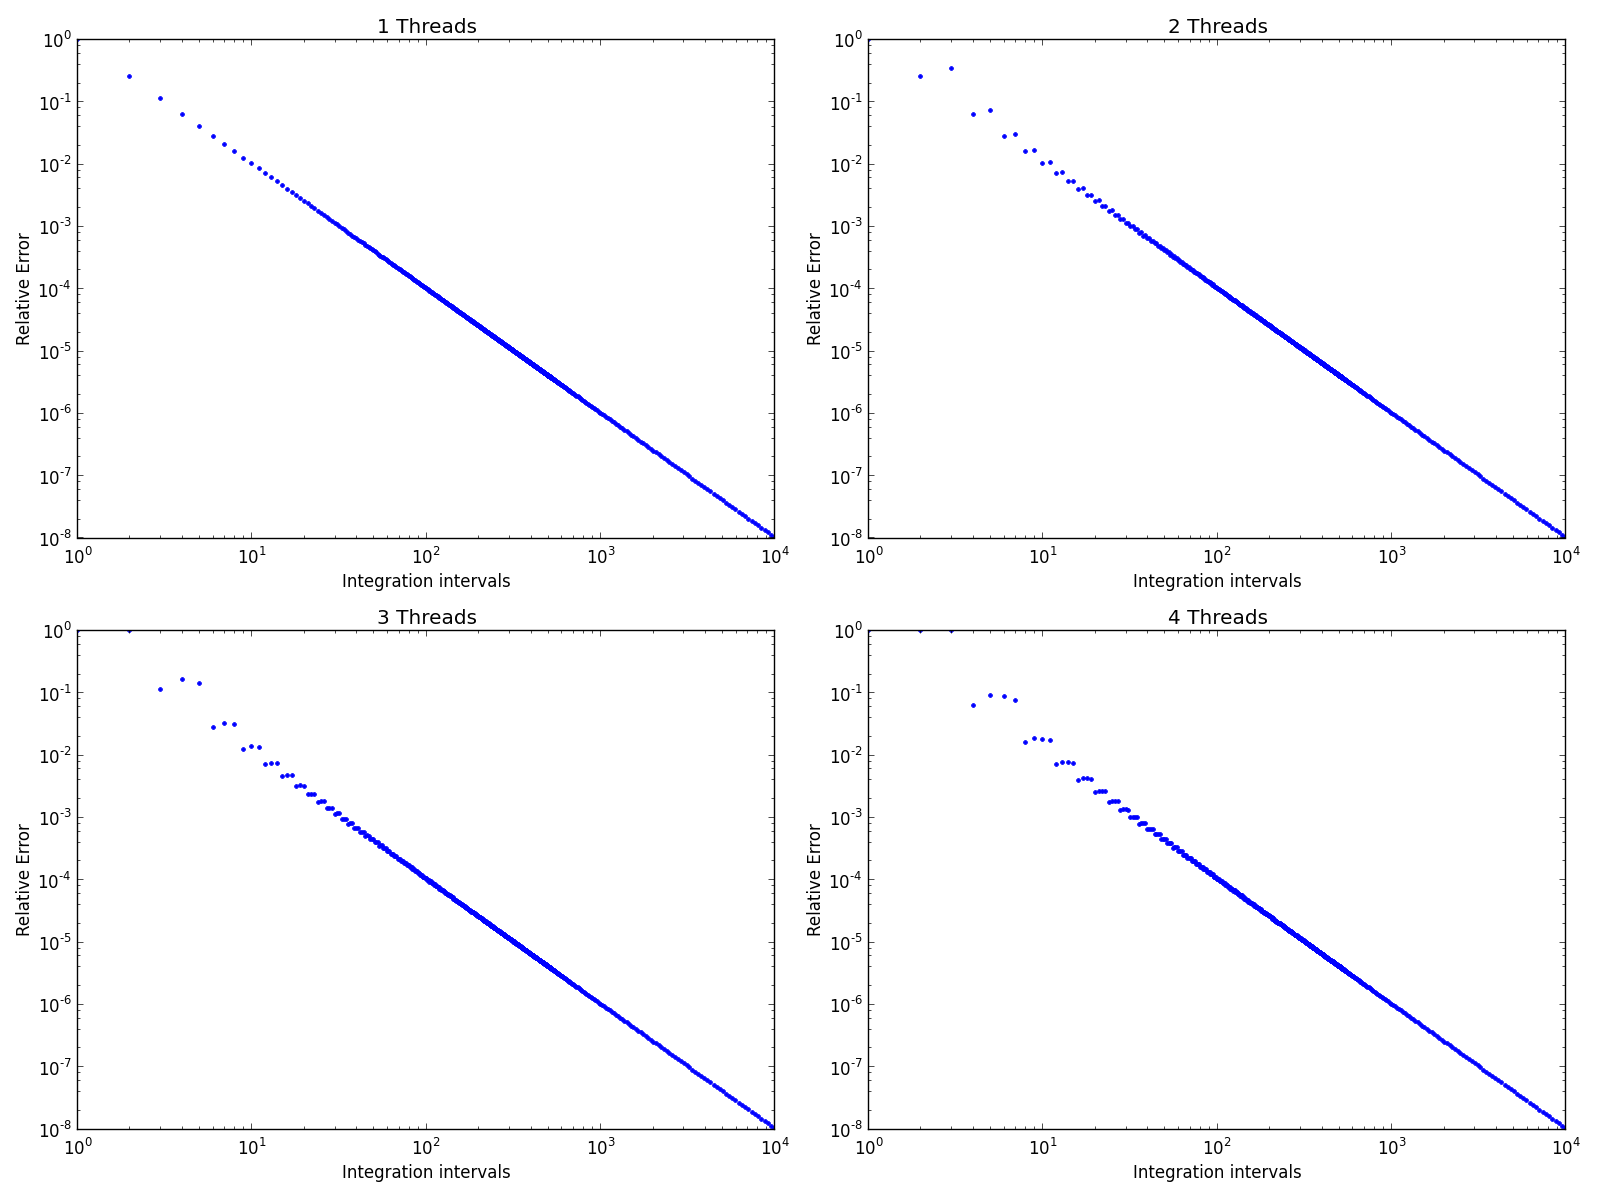
\includegraphics[width=\linewidth]{../02/RelativeErrorCenter.pdf}
	\end{minipage}
	\captionof{figure}{Der relative Fehler in Abhängigkeit von der Intervallanzahl für verschiedene Anzahl von Threads ergo Teilintervallen}
	\label{fig:RelativeErrorCenter}
\end{center}

(!!!)
Der relative Fehler in Abhängigkeit von der Intervallanzahl. Die einzigen Fehler, die durch die Parallelisierung entstehen könnten sind FloatingPoint-Fehler der Art: $(a+b)+c \neq a + (b+c)$, aber diese sind auf Niveau von FLT\_EPSILON bzw. DBL\_EPSILON und damit nur für das Minimum in Abb.\ref{fig:RelativeError} relevant.\\

\begin{center}
	\captionsetup{type=figure}
	\centering
	\begin{minipage}{0.7\linewidth}
		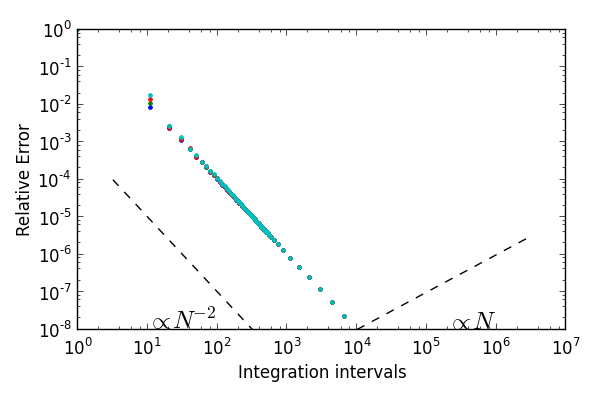
\includegraphics[width=\linewidth]{../02/RelativeError.pdf}
	\end{minipage}
	\captionof{figure}{Der relative Fehler der numerischen Integration mittels Mittelpunktregel und mittels Trapezregel, erstere auch für 'float' durchgeführt von einem Thread}
	\label{fig:RelativeError}
\end{center}

Bis rund 1000 Integrationsintervalle sinkt der Fehler immer weiter bis ungefähr auf FLT\_EPSILON= 1.19209290E-07 ab. Es gibt einige interessante Ausnahmen, die bis auf DBL\_EPSILON absinken. Da die Berechnung des relativen Fehlers und auch das MPI\_REDUCE trotzdem mit 'double' arbeitet kann es vorkommen, dass nach typecasting und anderen Rechenoperationen durch Zufall der richtige Werte auch mit double precision getroffen wird. (Einen Einzelfall raussuchen und Schritt für Schritt aufschlüsseln!!! -> MPI\_Reduce ist leider ne Blackbox)\\
Für mehr als 1000 Intervalle beginnt der Fehler wieder anzusteigen, weil die Intervallbreite sich FLT\_EPSILON annähert und damit FloatingPoint-Fehler einführt. Auch die Funktionswerteberechnung selber hat nur eine bestimmte Präzision, sodass allein dadurch der Integrationsalgorithmus auf einer Art Stufenfunktion arbeitet. (Das sollte aber nur zu einem sättigendem Verlauf führen??? Doch nochmal ganz genau überlegen mit Bleistift und Papier ... Taylor-Entwicklung und Co machen !!! nochmal versuchen den $h^{-1}$ Fehler zu erklären)\\

% Copy paste aus hausaufgabe im 5. Semester


%Das Ergebnis wird für kleinere h nicht mehr besser, weil Rundungsfehler auftreten. Auf h ist kein Rundungsfehler, da es bei 0 liegt und somit beliebig kleine h durch (fast) beliebig kleinen Exponenten gespeichert wreden können. Der Rundungsfehler muss also in der Funktionsberechnung auftreten: 
%    1/h*( f(x0+h)+f(x0) ) wird zu
%    1/h (f(x0+h)+-err + f(x0)+-err) wird zu (Maximalfehler)
%    1/h (f(x0+h)+ f(x0)) +-err/h
%Hierbei ist err=1e-16 der Fehler, der aufgrund der endlichen Groesse (52 Bit)
%der Mantisse bei double (precision floating point number) auftritt.
%Ueber Taylor-Entwicklung wurde in der Vorlesung der Fehler aus dem Algorithmus
%selber abgeschaetzt auf O(h). Das ergibt also einen Gesamtwert:
%    A(x0) = f'(x0) + O(h) + O(err/h)
%Analog zu Experimentierfehlern ist es am guenstigen falls O(h)=O(err/h), also
%fuer h=err/h <=> h=Sqrt[err] = 10e-8. Das deckt sich sehr gut mit der Fehler-
%kurve der Vorwaertsdifferentiation, die bei ca.10e-8 ihr Minimum hat.
%Daraus dass fuer kleine h die Fehlerkurven aller 3 Methoden das gleiche
%asymptotische Verhalten aufweisen, kann man schlussfolgern, dass es sich wohl
%wahrscheinlich um diesselbe Fehlerursache bei kleinen h handelt, also nicht
%aus dem Algorithmus sondern wie beschrieben aus der Rundung kommt.
%Bis auf Verschiebungen, die egal sind, stimmt das Verhalten der Fehlerkurven
%fuer groessere h auch sehr gut mit den Fehlern ueberein, die mit Taylor fuer
%den Algorithmus berechnet wurden.
%A similiar argumentation gives us the extrema for the other methods:
%    h_fwd = 1e-8
%    h_cnt = 1e-16/3 = 1e-5.333 = 5e-6
%    h_ext = 1e-16/5 = 1e-3.2 = 6e-4
%Only h_ext deviates a tad from the observed minimum at 1.5e-3. This could
%be a dependance of the differentiated function.
%Approximate minimal relative errors as displayed in the plot:
%    err_min_fwd = 1e-8
%    err_min_cnt = 1e-11
%    err_min_ext = 1e-13
%"""

(!!!) Vermutung: da die Anzahl der Einzelurven mit der Anzahl der Threads steigt, könnte es ein modulo-problem geben. Also dass der relative Fehler nur dann schlecht ist, wenn 7 Intervalle auf 3 Threads verteilt werden müssen z.b.. Wo liegen die x-Werte der Kurven?
Dem ist in der Tat so. z.b. in '2014-11-3\_0-56-data.txt' ab Zeile 1478. Werte auf oberer Kurve/hohen Fehlern:\\
\begin{tabular}{|c|c|c|c|c|c|c|c|c|c|c|c|c|c|c|c|}
	\hline
	77 &    &    & 80 &    &    & 83 &    &    & 86 &    &    & 89 &    &    \\
	\hline
	   & 78 & 79 &    & 81 & 82 &    & 84 & 85 &    & 87 & 88 &    & 90 & 91 \\
	\hline
\end{tabular}
Der Fehler ist also besonders schlecht, wenn ein Thread 2 Threads 1 Intervall mehr haben sollten als der dritte.\\

Berechnung Nbeforeme war falsch! oder das locN hätte nach nBeforeme incrementiert werden müssen...Jetzt geht alles

%%%%%%%%%%%%%%%%%%%%%%%%%%%%%%%%%%%%%%%%%%%%%%%%%%%%%%%%%%%%%%%%%%%%%%%%%%%%

http://maxinator.bplaced.net/share/MatrixCache.png

Das sind die Gigaflop in abhängigkeit von der Matrix-größe in Bytes. DIe schwarzen senkrechten linien sind die Cachegrößen des Taurus-Nodes: L1:32k, L2:256kb und L3 20MB. Man sieht also schön, wie die Gigaflops runtergehen, wenn er nicht mehr die komplette Matrix in den Speicher quetschen kann. Was jetzt noch fehlt ist ein Vergleich mit Blocking. Da sollte das dann ab dem L3-Cache nicht mehr abfallen.


\newpage

\printbibliography

\end{document}
